\documentclass[zihao=false,fontset=windows]{ctexart}
% ctexart 不接受任意 pt 选项。正文改 {10pt}，方括号里是行距。
\usepackage{scrextend}
\changefontsizes[12pt]{10pt}

\usepackage[a4paper,left=2.35cm,right=2.35cm,top=1.7cm,bottom=1.9cm]{geometry}
\usepackage{xcolor}
\usepackage{graphicx}
\usepackage{amsmath,amssymb}
\usepackage{enumitem}
\usepackage{tabularx}
\usepackage{colortbl}
\usepackage{listings}
\usepackage{hyperref}
\usepackage[most]{tcolorbox}

\definecolor{feishuText}{RGB}{31,35,41}
\definecolor{feishuBlue}{RGB}{36,91,219}
\definecolor{feishuRed}{RGB}{216,57,49}
\definecolor{feishuGray}{RGB}{100,106,115}
\definecolor{feishuGray2}{RGB}{143,149,158}
\definecolor{feishuPinkBg}{RGB}{251,191,188}
\definecolor{quoteBar}{RGB}{51,112,255}
\definecolor{codebg}{RGB}{245,246,247}
\definecolor{codeborder}{RGB}{222,224,227}
\definecolor{inlinebg}{RGB}{242,243,245}
\definecolor{callRed}{RGB}{253,226,226}
\definecolor{callOrange}{RGB}{255,245,235}
\definecolor{callYellow}{RGB}{254,255,240}
\definecolor{callGreen}{RGB}{240,251,239}
\definecolor{callBlue}{RGB}{240,244,255}
\definecolor{callRedSoft}{RGB}{254,241,241}
\definecolor{callSun}{RGB}{255,255,204}
\definecolor{tableHead}{RGB}{242,243,245}
\definecolor{tableRule}{RGB}{222,224,227}
\definecolor{codeText}{RGB}{31,35,41}
\definecolor{codeKeyword}{RGB}{0,0,255}
\definecolor{codeComment}{RGB}{0,128,0}
\definecolor{codeString}{RGB}{163,21,21}

\setmainfont{Times New Roman}
\setCJKmainfont{Microsoft YaHei}[AutoFakeBold=2.2]
\setCJKsansfont{Microsoft YaHei}[AutoFakeBold=2.2]
\setCJKmonofont{Microsoft YaHei}[AutoFakeBold=2.2]
\setmonofont{Consolas}
\newfontfamily\emojifont{Segoe UI Emoji}

\hypersetup{
  colorlinks=true,
  urlcolor=feishuBlue,
  linkcolor=feishuBlue,
  unicode=true,
  pdftitle={DeepSeek-V4.1-Flash 预训练/后训练解析}
}

\setlength{\parindent}{0pt}
\setlength{\parskip}{0.42em}
\setlength{\fboxsep}{1.5pt}
\setlength{\emergencystretch}{3em}
\linespread{1.28}
\color{feishuText}
\arrayrulecolor{tableRule}
\urlstyle{same}

\setlist[enumerate]{label=\textcolor{feishuBlue}{\arabic*.}, leftmargin=1.7em, itemsep=0.22em, topsep=0.28em, parsep=0.08em, partopsep=0pt}
\setlist[itemize,1]{label=\textcolor{feishuBlue}{\textbullet}, leftmargin=1.35em, itemsep=0.18em, topsep=0.25em, parsep=0.06em, partopsep=0pt}
\setlist[itemize,2]{label=\textcolor{feishuBlue}{◦}, leftmargin=1.45em, itemsep=0.12em, topsep=0.15em}
\setlist[itemize,3]{label=\textcolor{feishuBlue}{\rule[0.18em]{0.38em}{0.38em}}, leftmargin=1.55em, itemsep=0.1em, topsep=0.12em}

\newcommand{\feiEmoji}[1]{{\emojifont #1}}
\newcommand{\incode}[1]{\colorbox{inlinebg}{\ttfamily\small #1}}
\newcommand{\bigmath}[1]{%
  \begin{center}\large$\displaystyle #1$\end{center}%
}

\lstset{
  language=Python,
  basicstyle=\ttfamily\footnotesize\color{codeText},
  keywordstyle=\color{codeKeyword},
  commentstyle=\color{codeComment},
  stringstyle=\color{codeString},
  showstringspaces=false,
  breaklines=true,
  columns=fullflexible,
  keepspaces=true,
  tabsize=4,
  upquote=true,
  aboveskip=2pt,
  belowskip=0pt,
  xleftmargin=0pt,
  frame=none
}

\tcbset{
  feishubase/.style 2 args={
    enhanced,
    boxrule=0pt,
    arc=8pt,
    left=10pt,
    right=10pt,
    top=7pt,
    bottom=7pt,
    before skip=6pt,
    after skip=6pt,
    colback=#1,
    colframe=#1,
    before upper={\feiEmoji{#2}\hspace{0.45em}\ignorespaces}
  }
}
\newtcolorbox{feishubox}[2]{feishubase={#1}{#2}, breakable}
\newtcolorbox{feishuboxnb}[2]{feishubase={#1}{#2}}

\newtcolorbox{feishuquote}{
  enhanced,
  breakable,
  boxrule=0pt,
  leftrule=3pt,
  arc=0pt,
  colframe=quoteBar,
  colback=white,
  left=8pt,
  right=2pt,
  top=2pt,
  bottom=2pt,
  before skip=4pt,
  after skip=4pt,
  before upper=\color{feishuGray}
}

\newtcolorbox{feishucode}{
  enhanced,
  breakable,
  colback=codebg,
  colframe=codeborder,
  boxrule=0.6pt,
  arc=6pt,
  left=6pt,
  right=6pt,
  top=5pt,
  bottom=4pt,
  before skip=6pt,
  after skip=6pt
}


\usepackage{needspace,longtable,array,adjustbox}
% 来源：https://scnajei2ds6y.feishu.cn/wiki/JD1Lw2gLDiZYE1k3f23c6yo2nBf
% 按用户要求省略全部代码块；正文公式按网页渲染人工转写核对。
% 图108从页面已观察PNG资源导出；其他图与Pipeline白板以正常浏览器截图保留，详见复刻说明。
\begin{document}
{\zihao{1}\bfseries DeepSeek-V4.1-Flash 预训练/后训练解析\par}

% source-block: 2 doxcnAPvI7DwAIJUMPRXzGytPXe callout
\begin{feishubox}{callBlue}{📌}

% source-block: 3 doxcnAPsQOrGCNbiJv2XxVUbzcf text
\textbf{前置推荐阅读：}\par
\begin{itemize}
\item 
% source-block: 4 doxcnCvdMBlnD6whmUVOSBGBIKg bullet
\href{https://scnajei2ds6y.feishu.cn/wiki/StxKwYlBfi7D0DkwO0rcdjMInEZ}{DeepSeek-V4.1-Flash 架构：技术报告/源码解析}\par
\item 
% source-block: 5 doxcnGtA0IscWZLFoJCMImvKhgf bullet
\href{https://my.feishu.cn/wiki/C7KRwSCpZiE7olknCUPcKGY4n5c}{DeepSeek-V4 训练流程: Pretrain+Online Distillation}\par
\item 
% source-block: 6 doxcnIgY3YPPA6EBEoX1Kb3Z7Nb bullet
\href{https://scnajei2ds6y.feishu.cn/wiki/Hcj2wGTJEiohTikkdEKc7H4Nnlb}{Muon 优化器}\par
\item 
% source-block: 7 doxcnoQob7B3spC1bNL2fm8kBYb bullet
\href{https://scnajei2ds6y.feishu.cn/wiki/J5iOw7jRxi3tjSkNDSMcTJwmn5d}{\feiEmoji{🆕}On-Policy Distillation 是什么？工作脉络梳理 }\par
\item 
% source-block: 8 doxcnbzzsl8sQ0J7GloNtRoPlrg bullet
\href{https://my.feishu.cn/wiki/TaPYw0sGViHBFNkXdFIceLTWnEg?from=space_search}{\feiEmoji{📗}2026年基座模型中的 On-Policy Distillation 技术总结}\par
\end{itemize}
\end{feishubox}

% source-block: 9 doxcneFRjesg0WKu4B8C79aEetq callout
\begin{feishubox}{callOrange}{📌}

% source-block: 10 doxcn7u5vWa6rsVlUcXHdz6g6ue text
\textbf{技术报告：}\href{https://huggingface.co/deepseek-ai/DeepSeek-V4.1-Flash/blob/main/DeepSeek_V41_Tech_Report.pdf}{《DeepSeek-V4.1-Flash: Pushing the Limits of KV Cache Compression》}\par

% source-block: 11 doxcn21kRy6chEZvQXqNPmfZVzh text
\textbf{模型仓库：}\href{https://huggingface.co/deepseek-ai/DeepSeek-V4.1-Flash}{deepseek-ai/DeepSeek-V4.1-Flash}\par

% source-block: 12 doxcnfl0H5zPbLz7YweQl1Vdtzb text
\textbf{包含知识点：}\par
\begin{itemize}
\item 
% source-block: 13 doxcnsP5TbSfqtXPrR3NY8Wne5g bullet
\textbf{预训练：}45T 文本 + 多模态混合语料、直接训练 sparse attention（取消 DeepSeek V4 的 dense 冷启动）、DeepSeek-ViT 通过 contrastive pre-training + autoregressive fine-tuning 两阶段预训练。\par
\item 
% source-block: 14 doxcnoiNNNp727vBlrNea9v0fhT bullet
\textbf{后训练：}复用 V4 后训练 Pipeline，\textcolor{feishuRed}{不引入新的后训练算法}，投入在数据和环境 Scaling。包括大规模 Agent 任务-环境合成、Scaffold + Compute 的异步 RL Scaling、40+ Teacher full-vocabulary OPD。\par
\end{itemize}
\end{feishubox}

% source-block: 15 doxcncB2CGArzwQa6nPAoIs2Uvb heading2
\par\Needspace{8\baselineskip}\vspace{0.8em}\noindent \begin{tcolorbox}[boxrule=0pt,arc=3pt,colback=callRed,left=3pt,right=3pt,top=2pt,bottom=2pt,before skip=0pt,after skip=0pt]{\zihao{-2}\bfseries \textcolor{feishuBlue}{1.}\ 预训练（Pre-Training）}\end{tcolorbox}\par\vspace{0.28em}

% source-block: 16 doxcn8KAc69ulIi3PkzwhumCYAf quote_container
\begin{feishuquote}

% source-block: 190 doxcnqPfIuJeeQSNo6ui7tLRvNb text
前置阅读：\href{https://my.feishu.cn/wiki/C7KRwSCpZiE7olknCUPcKGY4n5c}{DeepSeek-V4 训练流程: Pretrain+Online Distillation}。\par

% source-block: 191 doxcn3Q94uwwPpNL1WdujXMkAMc text
DeepSeek V4 的数据配方、稳定性手段与 OPD 框架在上文已完整解析，下面主要关注 V4.1-Flash 的改进。\par
\end{feishuquote}

% source-block: 17 doxcn1Fi0ce114zL5FFHhFHnfAt text
V4.1-Flash 的预训练相对 V4 有三处结构性变化：\par
\begin{itemize}
\item 
% source-block: 18 doxcnDQ4jsNwGD4cAcKSTS8dbYd bullet
语料扩充到 45T token（文本与多模态混合）。\par
\item 
% source-block: 19 doxcnuY9WSg9bIs1he3reJjxO2f bullet
视觉编码器先单独两阶段（2-Stage）训练、再接入进行统一预训练。\par
\item 
% source-block: 20 doxcn4lGfTQs406sxNisP6U5dpf bullet
Embedding 参数切换优化器。\par
\end{itemize}

% source-block: 21 doxcnM4Y8HEA9Y4inE4hDoUTcOb heading3
\par\Needspace{8\baselineskip}\vspace{0.8em}\noindent \begin{tcolorbox}[boxrule=0pt,arc=3pt,colback=callOrange,left=3pt,right=3pt,top=2pt,bottom=2pt,before skip=0pt,after skip=0pt]{\zihao{3}\bfseries \textcolor{feishuBlue}{1.1}\ 训练数据}\end{tcolorbox}\par\vspace{0.28em}

% source-block: 22 doxcnFrQTJLk474fu0lpWri3zOP heading4
\par\Needspace{8\baselineskip}\vspace{0.8em}\noindent \begin{tcolorbox}[boxrule=0pt,arc=3pt,colback=callGreen,left=3pt,right=3pt,top=2pt,bottom=2pt,before skip=0pt,after skip=0pt]{\zihao{4}\bfseries \textcolor{feishuBlue}{1.1.1}\ 文本语料}\end{tcolorbox}\par\vspace{0.28em}
\begin{itemize}
\item 
% source-block: 23 doxcnhDuaL6wjZpnlaXkaA6cz0d bullet
\textbf{Scaling ladder}：在模型参数与训练数据维度上进行 Scaling 实验指导大规模训练的配比。\par
\item 
% source-block: 24 doxcn7v0waopcTrvmstSMsf1aUc bullet
\textbf{隐式重复（implicit duplication）}：过滤弱模型输出与低质量机翻文本。\par
\item 
% source-block: 25 doxcnOWMO1ilrkurqoaBK1NAUBD bullet
\textbf{代码时效}：补入新发布的开源仓库、commit、库与框架，覆盖更多编程语言。\par
\end{itemize}

% source-block: 26 doxcn6TGW37pOva6xeqKQq1cQoh heading4
\par\Needspace{8\baselineskip}\vspace{0.8em}\noindent \begin{tcolorbox}[boxrule=0pt,arc=3pt,colback=callGreen,left=3pt,right=3pt,top=2pt,bottom=2pt,before skip=0pt,after skip=0pt]{\zihao{4}\bfseries \textcolor{feishuBlue}{1.1.2}\ 多模态语料}\end{tcolorbox}\par\vspace{0.28em}

% source-block: 27 doxcnNFqEEXQLWXGvM1rKx2UoPd text
多模态预训练数据分图文 pair、图文交错、领域数据三类，\textcolor{feishuRed}{V4.1-Flash 论文认为网页原生数据已含丰富的多模态知识，因此明确不做大规模合成，直接清洗使用。}\par
\begin{itemize}
\item 
% source-block: 28 doxcnn0qwDy5f4PAiEQbtbfkKtc bullet
\textbf{爬虫重置}：初始爬取系统偏向纯文本网页，改从 Common Crawl 重新 bootstrap。\par
\item 
% source-block: 29 doxcn5HW5h6bdBi1YhPD1emYOLf bullet
\textbf{图文 pair}：抽取网页图片与 alt text，按图文相关性阈值过滤，按图像语义去重。\par
\item 
% source-block: 30 doxcnCGVhSE0eqI7OxPFPJBYxKc bullet
\textbf{领域数据}：visual grounding 与 pointing、OCR、长尾知识，以及 image-code 对与 computer-use 轨迹。\par
\end{itemize}

% source-block: 31 doxcnLEUJFs2ltFWneTOKCFqPhb text
图文交错数据主要来自网页与 PDF，处理成本高于纯文本，因此按成本递增分三级处理：\par
\begin{enumerate}
\item 
% source-block: 32 doxcnL4wvJqL59XpGSxygjysk7f ordered
拉取图片之前，用启发式与统计过滤、去重、质量模型挑出高价值文档。\par
\item 
% source-block: 33 doxcnApK9eFCh3BItk6B6TLORvb ordered
组装成图文交错序列，再做图像感知的过滤与去重。\par
\item 
% source-block: 34 doxcnqYRbqnbNVboW3Po88SFC7e ordered
用 SmolVLM 对图文内容严格打分，被筛掉的文档部分回收成图文对。\par
\end{enumerate}

% source-block: 35 doxcnrCgRzCxjnGoFiMG3FWTvwi heading4
\par\Needspace{8\baselineskip}\vspace{0.8em}\noindent \begin{tcolorbox}[boxrule=0pt,arc=3pt,colback=callGreen,left=3pt,right=3pt,top=2pt,bottom=2pt,before skip=0pt,after skip=0pt]{\zihao{4}\bfseries \textcolor{feishuBlue}{1.1.3}\ Merge / Packing}\end{tcolorbox}\par\vspace{0.28em}
\begin{itemize}
\item 
% source-block: 36 doxcnIqWw2K5gAdSCtgzbvPGpLc bullet
文本与多模态重叠样本用多模态版本替换纯文本版本，替换后纯文本与多模态的 token 比是 7:1。\par
\item 
% source-block: 37 doxcnpReZvIfYOfJtsPhGDQnn7c bullet
预训练与上下文扩展阶段联合预取并分配样本，尽量减少样本重叠。\par
\item 
% source-block: 38 doxcnpStKaTUeYaHL0cWL6Of2Ld bullet
超长文档在混合前确定性切分，使训练 token 在各数据分片与训练步之间分布均匀。\par
\item 
% source-block: 39 doxcnqAPQ09Z6a5rswT0p3NynCc bullet
预训练使用 sample-level attention masking。\par
\end{itemize}

% source-block: 40 doxcnp5I0STOyxlJelpLz0RfwNf heading3
\par\Needspace{8\baselineskip}\vspace{0.8em}\noindent \begin{tcolorbox}[boxrule=0pt,arc=3pt,colback=callOrange,left=3pt,right=3pt,top=2pt,bottom=2pt,before skip=0pt,after skip=0pt]{\zihao{3}\bfseries \textcolor{feishuBlue}{1.2}\ 训练配置}\end{tcolorbox}\par\vspace{0.28em}

% source-block: 41 doxcnFpZHxNCYiFHudJu3I5Nj7c text
整个预训练过程中学习率、序列长度与 ViT 冻结状态随 Token 训练数量的设置：\par

% source-block: 42 doxcnfl5B74H7tYPqxkrVhkVlHf image
\begin{center}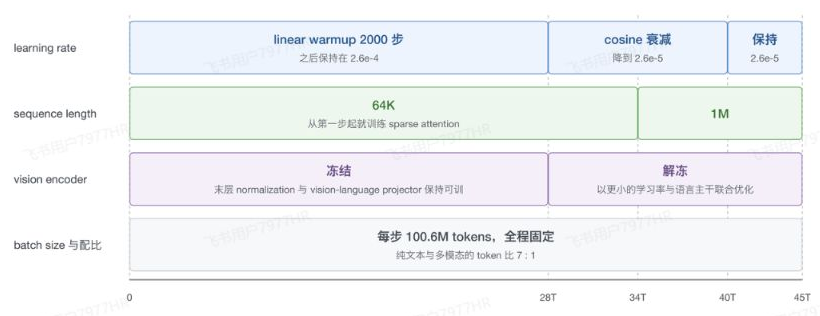
\includegraphics[width=0.98\linewidth,height=0.82\textheight,keepaspectratio]{images/DeepSeek-V4.1-Flash训练/doxcnfl5B74H7tYPqxkrVhkVlHf.png}\end{center}
\begin{itemize}
\item 
% source-block: 43 doxcnESyROmbLZohUeonynv8rdb bullet
稀疏注意力去掉冷启动：\par
\begin{itemize}
\item 
% source-block: 192 doxcn23ilVPBdA6ptlCQ3kxf8ac bullet
DeepSeek V4 先用 dense attention 适应 64K 上下文，再做 indexer warmup，最后切换稀疏注意力。\par
\item 
% source-block: 193 doxcnZMhim3vhBhM2kxvYRTzFlc bullet
V4.1-Flash 直接在 64K 上下文训练稀疏注意力。\par
\end{itemize}
\item 
% source-block: 44 doxcnwlxTKyPxznoXwWA3Lv7AVd bullet
稳定性部分去掉 DeepSeek V4 的 \href{https://my.feishu.cn/wiki/C7KRwSCpZiE7olknCUPcKGY4n5c\#share-V2PLdReFUoGXTCxTAvBcSM5bnSh}{Anticipatory Routing}。\par
\item 
% source-block: 45 doxcnC35ChpGcDRldlxj8ArsKBf bullet
沿用 DeepSeek V4 的 SwiGLU Clamping。\par

% source-block: 194 doxcnJHIgs6rinH1DTwsLYzT1Ad code
% Code block omitted at user request.
\item 
% source-block: 46 doxcnxhdlXS3UNNmQXunKPwnaXd bullet
64K 的上下文扩展到 1M 的上下文需要 YaRN 外推，外推倍数 \incode{rope\_factor = 16}：\par

% source-block: 195 doxcnezSLdmLLg5rj83xwrjKSNd code
% Code block omitted at user request.

% source-block: 196 doxcniRyqwxUtl0J1qMtgMiLhdh text
\incode{compress\_ratio} 为 0 的层（第 0、1 层与 DSpark 层）不使用外推，用基础 rope\_theta。\par
\end{itemize}

% source-block: 47 doxcn1SF4smkvQrGaO38XO5xh9b heading3
\par\Needspace{8\baselineskip}\vspace{0.8em}\noindent \begin{tcolorbox}[boxrule=0pt,arc=3pt,colback=callOrange,left=3pt,right=3pt,top=2pt,bottom=2pt,before skip=0pt,after skip=0pt]{\zihao{3}\bfseries \textcolor{feishuBlue}{1.3}\ 优化器}\end{tcolorbox}\par\vspace{0.28em}

% source-block: 48 doxcn5m6GwietpSN53UC9rCbKKf quote_container
\begin{feishuquote}

% source-block: 197 doxcndvqHHPQ44yYTuuVmImxXfb text
推荐前置阅读：\href{https://scnajei2ds6y.feishu.cn/wiki/Hcj2wGTJEiohTikkdEKc7H4Nnlb}{Muon 优化器}\par
\end{feishuquote}

% source-block: 49 doxcn5axNDmf2JIHUPZpXy1MzXd heading4
\par\Needspace{14\baselineskip}\vspace{0.8em}\noindent \begin{tcolorbox}[boxrule=0pt,arc=3pt,colback=callGreen,left=3pt,right=3pt,top=2pt,bottom=2pt,before skip=0pt,after skip=0pt]{\zihao{4}\bfseries \textcolor{feishuBlue}{1.3.1}\ 参数分组优化}\end{tcolorbox}\par\vspace{0.28em}

% source-block: 50 doxcnX20SIDMDZiNgtMZvvcJuqc table
\begin{longtable}{|>{\raggedright\arraybackslash}p{4.6cm}|>{\raggedright\arraybackslash}p{4.6cm}|>{\raggedright\arraybackslash}p{4.6cm}|}\hline
\rowcolor{tableHead} 
% source-block: 199 doxcnPiEdBuNOMDRKqNqtuP7QV3 text
\textbf{参数组}\par
 & 
% source-block: 201 doxcnlSX2tELPN77wrphvV9CQhc text
\textbf{优化器}\par
 & 
% source-block: 203 doxcn9ubSxhPNpztGaBPWEInI0g text
\textbf{超参数}\par
 \\ \hline
\endfirsthead
\hline\rowcolor{tableHead} 
% source-block: 199 doxcnPiEdBuNOMDRKqNqtuP7QV3 text
\textbf{参数组}\par
 & 
% source-block: 201 doxcnlSX2tELPN77wrphvV9CQhc text
\textbf{优化器}\par
 & 
% source-block: 203 doxcn9ubSxhPNpztGaBPWEInI0g text
\textbf{超参数}\par
 \\ \hline
\endhead

% source-block: 205 doxcnUpfuDOeRrajyb2jufxPZBg text
\textbf{RMSNorm 权重、bias、缩放因子等非矩阵参数}\par
 & 
% source-block: 207 doxcnSQYGf83sJ9PI2h8fHIQ4eg text
\textbf{AdamW}\par
 & 
% source-block: 209 doxcnmWRroDIzwmBbZaHfN7OzVg text
$\beta_1=0.9$、$\beta_2=0.95$、$\varepsilon=10^{-20}$、weight decay 0.1。weight decay 只施加在 norm 权重上，bias 与缩放因子不施加。\par
 \\ \hline

% source-block: 211 doxcnZ3LyXLf53Bg5hXkmQRrsch text
\textbf{主干线性变换权重、Engram 的 projection layers、vision-language projector}\par
 & 
% source-block: 213 doxcnDZ2F0yBlky1yWw8w1vahYd text
\textbf{Muon}\par

% source-block: 214 doxcnlPTjnrvHpUO33kQEz9Ekad text
 & 
% source-block: 216 doxcnwT3CiPEhcYNZvA161MMlTc text
momentum 0.95、weight decay 0.1，用 Nesterov momentum 与 decoupled weight decay。每个更新矩阵的 RMS 缩放到 0.18，以复用 AdamW 的 LR 经验值。\par
 \\ \hline

% source-block: 218 doxcngXjBDODRO1mobaMIrBLM3d text
\textbf{Query/Key 权重}\par
 & 
% source-block: 220 doxcnmVOYxp9og4m4wy7d5jt3dg text
\textbf{head-wise Muon}\par
 & 
% source-block: 222 doxcnDcZCQvnL6BLdwaHscB0fvd text
正交化按 head 分别做。\par
 \\ \hline

% source-block: 224 doxcnkaXWNWULbRJftEWIYcshNd text
\textbf{全部 Embedding 与 prediction head}\par
 & 
% source-block: 226 doxcnrwl8Ir0r1fIg8VjSkbR5Hh text
\textbf{Sinkhorn-balanced update}\par
 & 
% source-block: 228 doxcne6EqMpffhuBrWa8TQr8ECb text
Nesterov momentum、不施加 weight decay，LR 修正系数同 Muon，$K=11$、$\tau=10^{-3}$、$\varepsilon=10^{-20}$。Engram 的 LR 放大 5 倍。\par
 \\ \hline
\end{longtable}

% source-block: 51 doxcntB8DPgCpCS8tRiLt1SLHfc heading4
\par\Needspace{8\baselineskip}\vspace{0.8em}\noindent \begin{tcolorbox}[boxrule=0pt,arc=3pt,colback=callGreen,left=3pt,right=3pt,top=2pt,bottom=2pt,before skip=0pt,after skip=0pt]{\zihao{4}\bfseries \textcolor{feishuBlue}{1.3.2}\ Sinkhorn-Balanced Update}\end{tcolorbox}\par\vspace{0.28em}

% source-block: 52 doxcnudZmI3q6IkBbbMsSg6PZZc text
Embedding 这类大矩阵参数的优化器保留 Muon 的骨架，把 Newton-Schulz 正交化替换为 Sinkhorn balancing（交替做行归一与列归一，逼近双随机矩阵）：\par

% source-block: 53 doxcnou1VhNRMqfCVEQyyTrP0vf text
\bigmath{\begin{aligned}\Delta_t&=\sqrt{n}U^{(K)}=\sqrt{n}D_r\widehat{G}_tD_c,\\ \frac{1}{n}\sum_{j=1}^{n}(\Delta_t)_{ij}^{2}&\approx1,\qquad \frac{1}{m}\sum_{i=1}^{m}(\Delta_t)_{ij}^{2}\approx1\end{aligned}}
\begin{itemize}
\item 
% source-block: 54 doxcnBpxZnadW9ZI8p11Y5lV9Nh bullet
$W_t\in\mathbb{R}^{m\times n}$ 是参数矩阵，embedding table 和 output head 的 $m$ 是 vocab size，$n$ 是 hidden dim。\par
\item 
% source-block: 55 doxcnobzpKdjge6hg9vA6lvYMlc bullet
$\widehat{G}_t$ 是 Nesterov momentum 更新，$U^{(K)}$ 是 $K$ 步交替归一后的矩阵：奇数步按行、偶数步按列除以 $\ell_2$ 范数。\par
\item 
% source-block: 56 doxcnz3pL83ZF4gSg2o5lc4di8t bullet
$D_r$、$D_c$ 是归一化累积出来的对角缩放矩阵，$\sqrt{n}$ 负责把逐元素均方拉回 1 的量级。\par
\end{itemize}

% source-block: 57 doxcnklTfSWN9Gk2ZkUlqZoEu2c image
\begin{center}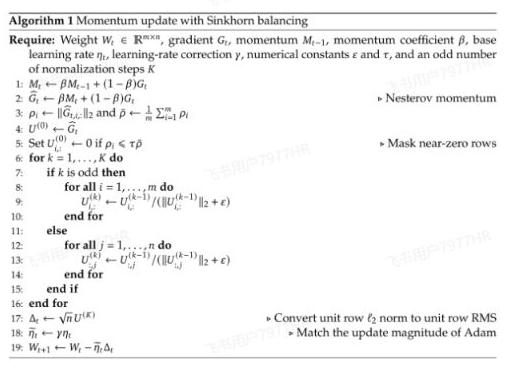
\includegraphics[width=0.98\linewidth,height=0.82\textheight,keepaspectratio]{images/DeepSeek-V4.1-Flash训练/doxcnklTfSWN9Gk2ZkUlqZoEu2c.png}\end{center}

% source-block: 58 doxcnGXrn8WOi4mPK9fdLDix2qe text
本质上这是用行列双随机的近似替换正交化。Newton-Schulz 要求整个矩阵接近正交，代价随 $m$（vocab size）增长。Sinkhorn 只要求行方向、列方向的均方各自约为 1，$K=11$ 步即可收敛，显存开销只存 momentum。\par

% source-block: 59 doxcnzFTe7LYWYv6vEr6hK0v14c heading3
\par\Needspace{8\baselineskip}\vspace{0.8em}\noindent \begin{tcolorbox}[boxrule=0pt,arc=3pt,colback=callOrange,left=3pt,right=3pt,top=2pt,bottom=2pt,before skip=0pt,after skip=0pt]{\zihao{3}\bfseries \textcolor{feishuBlue}{1.4}\ 视觉编码器 DeepSeek-ViT 训练}\end{tcolorbox}\par\vspace{0.28em}

% source-block: 60 doxcnTl5bSxXwVGsqpX1tGzQxYc quote_container
\begin{feishuquote}

% source-block: 229 doxcncBnPkHIZ1ukxB18yuxt8Ah text
前置阅读：\href{https://scnajei2ds6y.feishu.cn/wiki/IAqAwbiLVi0gEOkC87Qc0hAVnPe}{SigLIP}\par
\end{feishuquote}

% source-block: 61 doxcnKRiQV8IQuAPPHKM8k0w7Rc text
DeepSeek-ViT 在接入语言主干之前单独两阶段训练：对比预训练（Contrastive pre-training）、自回归微调（Autoregressive fine-tuning）：\par

% source-block: 62 doxcnIONKLFFiZtMjJj8lfMgQ7e image
\begin{center}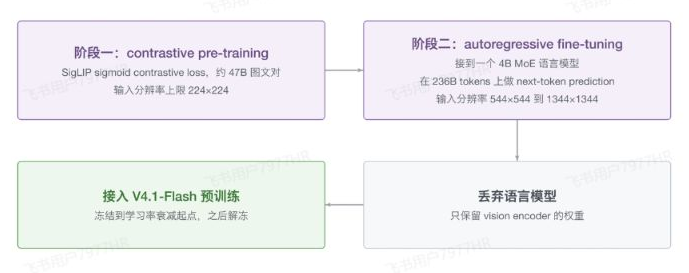
\includegraphics[width=0.98\linewidth,height=0.82\textheight,keepaspectratio]{images/DeepSeek-V4.1-Flash训练/doxcnIONKLFFiZtMjJj8lfMgQ7e.png}\end{center}

% source-block: 63 doxcnt4M6yNsNaKVMVI8cXShutb heading4
\par\Needspace{8\baselineskip}\vspace{0.8em}\noindent \begin{tcolorbox}[boxrule=0pt,arc=3pt,colback=callGreen,left=3pt,right=3pt,top=2pt,bottom=2pt,before skip=0pt,after skip=0pt]{\zihao{4}\bfseries \textcolor{feishuBlue}{1.4.1}\ 对比预训练（Contrastive pre-training）}\end{tcolorbox}\par\vspace{0.28em}
\begin{itemize}
\item 
% source-block: 64 doxcn8HDKTUjrCwRfYsEU61Lrah bullet
损失是 SigLIP 的 sigmoid 对比损失，数据是约 47B image-text pairs。\par
\item 
% source-block: 65 doxcni7MD70dEfbKz2OO5O9hyHg bullet
输入分辨率上限 224$\times$224，更大的图等比缩小。\par
\end{itemize}

% source-block: 66 doxcnNecr8mNleoDOivNgPVr0hd quote_container
\begin{feishuquote}

% source-block: 230 doxcn2M992I5Z1aDqSQqz5uudrf text
分辨率上限压到 224$\times$224 的实测依据：论文观察到这一阶段用更高分辨率有明显收益，但在最终模型的收益很小，提高对比阶段的分辨率于是只增加计算开销，整体改进有限。\par
\end{feishuquote}

% source-block: 67 doxcnsH8lMOvIbjWJFstmUOwysM text
同期 \href{https://scnajei2ds6y.feishu.cn/wiki/OOC2wZ3npiGJSIk1YvNcW83Mnvg}{Kimi K3 训练流程解析：多模态预训练 + 后训练（冷启动 Agentic SFT + 多专家 RL + MOPD） } 的 MoonViT-V2 走相反路线，不做 SigLIP 式对比预训练，直接用语言建模损失从头训练。\par

% source-block: 68 doxcnQq6YWkpIjsGbgx2GMeNeng heading4
\par\Needspace{8\baselineskip}\vspace{0.8em}\noindent \begin{tcolorbox}[boxrule=0pt,arc=3pt,colback=callGreen,left=3pt,right=3pt,top=2pt,bottom=2pt,before skip=0pt,after skip=0pt]{\zihao{4}\bfseries \textcolor{feishuBlue}{1.4.2}\ 自回归微调（Autoregressive fine-tuning）}\end{tcolorbox}\par\vspace{0.28em}
\begin{itemize}
\item 
% source-block: 69 doxcnBKSzEF5FClazhB1Nzyctld bullet
把第一阶段的 ViT 接入 4B MoE LLM，用 next-token prediction 在 236B token 上训练，数据包含 image caption / alt text / chart / OCR。\par
\item 
% source-block: 70 doxcnush7O8lXgcr5Ce9ildQQIb bullet
输入分辨率限定在 544$\times$544 到 1344$\times$1344 之间，超界图片等比缩放，后续预训练沿用同一策略。\par
\end{itemize}

% source-block: 71 doxcnfNCRTSkxhwAoLBEsNiErNd text
这一阶段的目标是增强 encoder 对细粒度视觉特征的建模能力。训练结束后丢弃 LLM，只保留 encoder 进入 pre-training，分辨率策略保持不变。\par

% source-block: 72 doxcnjXqR9XvDOudKuutMu2uHTd heading4
\par\Needspace{8\baselineskip}\vspace{0.8em}\noindent \begin{tcolorbox}[boxrule=0pt,arc=3pt,colback=callGreen,left=3pt,right=3pt,top=2pt,bottom=2pt,before skip=0pt,after skip=0pt]{\zihao{4}\bfseries \textcolor{feishuBlue}{1.4.3}\ 接入 pre-training}\end{tcolorbox}\par\vspace{0.28em}

% source-block: 73 doxcnYLnxE3P4mu5rOglVzp3Chc text
ViT 接入之后与 LLM 在同一个预训练里训练，ViT 一直冻结到 LR 衰减阶段，期间只有末层 norm 与 vision-language projector 保持可训。衰减一开始就解冻 ViT，用更小的学习率与 LLM 联合优化。\par

% source-block: 74 doxcnXwkddugVGhOBiDwOZy0Kjg heading3
\par\Needspace{8\baselineskip}\vspace{0.8em}\noindent \begin{tcolorbox}[boxrule=0pt,arc=3pt,colback=callOrange,left=3pt,right=3pt,top=2pt,bottom=2pt,before skip=0pt,after skip=0pt]{\zihao{3}\bfseries \textcolor{feishuBlue}{1.5}\ 预训练评估结果}\end{tcolorbox}\par\vspace{0.28em}

% source-block: 75 doxcnV1kJQsrbFfZq39Thvv8q40 text
在内部评测框架、统一设置下对比三个 base 模型：\par

% source-block: 76 doxcnJdwQOb9KSy666yhn4IZpYj image
\begin{center}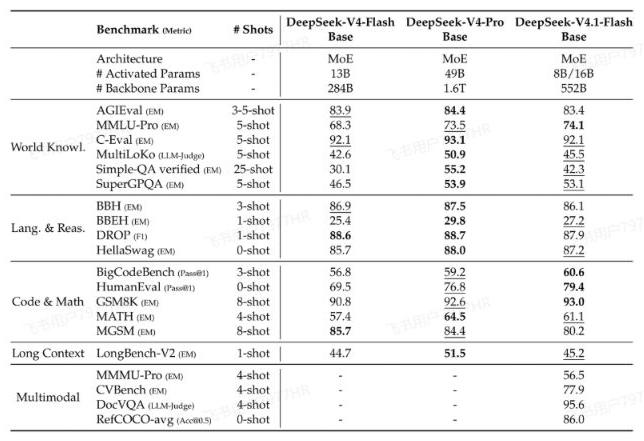
\includegraphics[width=0.98\linewidth,height=0.82\textheight,keepaspectratio]{images/DeepSeek-V4.1-Flash训练/doxcnJdwQOb9KSy666yhn4IZpYj.png}\end{center}

% source-block: 77 doxcn3rOAPUR4k80NFjhOnGzZsg text
重点看 V4.1-Flash-Base（8B/16B 激活）对比 V4-Pro-Base（49B 激活）：\par
\begin{itemize}
\item 
% source-block: 78 doxcnon90rSPIHHx7IArp9Y5Erf bullet
V4.1-Flash-Base 的激活参数远少于 V4-Pro-Base，KV cache 也大幅缩减，整体表现仍然持平：MMLU-Pro 74.1 vs 73.5、SuperGPQA 53.1 vs 53.9、HumanEval 79.4 vs 76.8。这意味着这一版的收益不只来自 token scaling，data pipeline 的改动在参数效率上同样有贡献。\par
\item 
% source-block: 79 doxcns18ti1NdlGiP828VuaqNNd bullet
但知识维度上对 V4-Pro 仍有明显差距，Simple-QA verified 42.3 vs 55.2、MultiLoKo 45.5 vs 50.9，说明知识容量这部分主要还是由激活参数量决定。\par
\end{itemize}

% source-block: 80 doxcnQzoNRz2O0nLbNGhCWGhpJe text

% source-block: 81 doxcnAkFNek7cCelp1GzBJyYivb heading2
\par\Needspace{8\baselineskip}\vspace{0.8em}\noindent \begin{tcolorbox}[boxrule=0pt,arc=3pt,colback=callRed,left=3pt,right=3pt,top=2pt,bottom=2pt,before skip=0pt,after skip=0pt]{\zihao{-2}\bfseries \textcolor{feishuBlue}{2.}\ 后训练（Post-Training）}\end{tcolorbox}\par\vspace{0.28em}

% source-block: 82 doxcnjRPuZ50XaK5X6kReKwb8lz quote_container
\begin{feishuquote}

% source-block: 83 doxcnRBNJ3fyjXaXlcD6Voaqyob text
\textbf{推荐前置阅读：}\par
\begin{enumerate}
\item 
% source-block: 84 doxcnqQJu8TF24BM4k9vk15I5j0 ordered
\href{https://scnajei2ds6y.feishu.cn/wiki/J5iOw7jRxi3tjSkNDSMcTJwmn5d}{\feiEmoji{🆕}On-Policy Distillation 是什么？工作脉络梳理 }\par
\item 
% source-block: 85 doxcnbMyKxLOToiYSeTzxTXSsKb ordered
\href{https://my.feishu.cn/wiki/C7KRwSCpZiE7olknCUPcKGY4n5c}{DeepSeek-V4 训练流程: Pretrain+Online Distillation}\par
\end{enumerate}
\end{feishuquote}

% source-block: 86 doxcnWooO1A01oE6G6A3KHWAare whiteboard
\begin{center}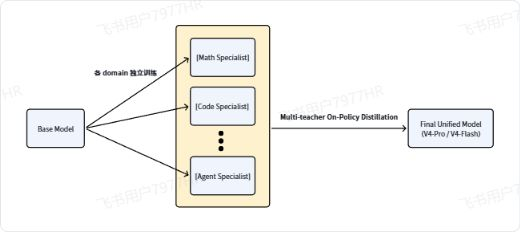
\includegraphics[width=0.98\linewidth]{images/DeepSeek-V4.1-Flash训练/pipeline-whiteboard.png}\par DeepSeek V4 后训练 Pipeline\end{center}

% source-block: 87 doxcneVHOL723wxrDEc0ODB2cJc text
DeepSeek-V4.1-Flash 的 post-training 仍然使用 \href{https://my.feishu.cn/wiki/C7KRwSCpZiE7olknCUPcKGY4n5c}{DeepSeek-V4} 的 SFT / RL / OPD 后训练路径，\textcolor{feishuRed}{\textbf{论文明确声明不引入新的后训练算法}}，投入几乎全部放在训练数据上而不是优化方式上：\par
\begin{itemize}
\item 
% source-block: 88 doxcn63GOMjwxU4fC2Eyk1NYund bullet
合成 diverse / verifiable 的训练任务，连同 reference solution 与 reward signal 产出。\par
\item 
% source-block: 89 doxcn7fBqf6V9e4DzgBB1PyRUQh bullet
程序化构建并扩展 interactive agent environment（Agent 能真实交互、结果可自动判定的环境），把 trajectory 的采集与评估成本压低。\par
\item 
% source-block: 90 doxcn6w9f2aZMKI2ARMVbivoYQc bullet
严格的 filtering、dedup、difficulty calibration，保证数据质量 / curriculum 平衡。\par
\end{itemize}

% source-block: 91 doxcnimzoPtbXe5nJDZ426dT2Rg quote_container
\begin{feishuquote}

% source-block: 92 doxcnPv4xbpt93Tw3jJdzLOQB2g text
V4.1 给出的判断是：在固定且普通的优化流程下，合成数据与环境在 scale / diversity / verifiability 上的系统性改进解释了几乎全部增益，这条路线的边际回报高于后训练的算法创新。\par
\end{feishuquote}

% source-block: 93 doxcnd6mRpU22ng66j7Du2oERGf heading3
\par\Needspace{8\baselineskip}\vspace{0.8em}\noindent \begin{tcolorbox}[boxrule=0pt,arc=3pt,colback=callOrange,left=3pt,right=3pt,top=2pt,bottom=2pt,before skip=0pt,after skip=0pt]{\zihao{3}\bfseries \textcolor{feishuBlue}{2.1}\ 大规模 Agent 任务合成}\end{tcolorbox}\par\vspace{0.28em}

% source-block: 94 doxcn1QlRRYIZBc16ZiyvdobSTY text
每个任务形式化成一个三元组 \incode{(problem, environment, verification system)}，质量由两个维度决定：\par
\begin{itemize}
\item 
% source-block: 95 doxcnkjpChm6xGBcLI2dYIicqUb bullet
\textbf{难度（difficulty）}：任务不能是平凡的。\par
\item 
% source-block: 96 doxcnpt3eiBowiaErUcTNUkhzhg bullet
\textbf{正确性（correctness）}：三个组件不含致命缺陷。\par
\end{itemize}

% source-block: 97 doxcndgqVxWbQoplAmbUnOqxXLf text
\textbf{关键设计点}：任务每进入一次新的 RL run，产出的 trajectory 反过来成为重新审计该任务的证据，质量控制因此覆盖任务的整个生命周期。\par

% source-block: 98 doxcnRKIWQuYYt8zFbPccdibuUd heading4
\par\Needspace{8\baselineskip}\vspace{0.8em}\noindent \begin{tcolorbox}[boxrule=0pt,arc=3pt,colback=callGreen,left=3pt,right=3pt,top=2pt,bottom=2pt,before skip=0pt,after skip=0pt]{\zihao{4}\bfseries \textcolor{feishuBlue}{2.1.1}\ General Agent}\end{tcolorbox}\par\vspace{0.28em}

% source-block: 99 doxcnxKOk4jo9p7EQq3BrGquMgc text
General Agent 的环境全部来自数据回收：\par
\begin{itemize}
\item 
% source-block: 100 doxcnNxdNiklOVm1frLNmuTrtdg bullet
\textbf{数据来源}：内部员工与外部合作方自愿把最新模型接入日常 workflow，回传交互数据与反馈。\par
\item 
% source-block: 101 doxcnV3uiigIPImBst9uDdotwpc bullet
\textbf{Mock 工具}：按回传数据里出现过的接口，复现真实工具的输入格式、输出结构、API schema、行为约束，覆盖常用 SaaS、企业应用与专门的业务后端系统。\par
\item 
% source-block: 102 doxcnbasnT4Dbg3njqg51JBYkNe bullet
\textbf{失败回放}：大规模收集 negative feedback 与失败案例，重建当时的 tool context、用户交互模式、失败条件，生成 single-turn 与 multi-turn 环境，针对已观测到的弱点做 RL。\par
\end{itemize}

% source-block: 103 doxcne3NpmrQ4AoP1uxMcrHBc8f heading4
\par\Needspace{8\baselineskip}\vspace{0.8em}\noindent \begin{tcolorbox}[boxrule=0pt,arc=3pt,colback=callGreen,left=3pt,right=3pt,top=2pt,bottom=2pt,before skip=0pt,after skip=0pt]{\zihao{4}\bfseries \textcolor{feishuBlue}{2.1.2}\ Coding Agent}\end{tcolorbox}\par\vspace{0.28em}

% source-block: 104 doxcnpJU4ZXM9AEpvLLK5PkdnKd text
Coding Agent 的环境来自两个来源：\par
\begin{itemize}
\item 
% source-block: 105 doxcnS7PkbOPvlvjuKDhD2mBk3f bullet
内部与外部合作 coding agent session（过滤后只保留高复杂度或模型表现差的任务，再按 trajectory dedup）。\par
\item 
% source-block: 106 doxcnOL8whbOCypgNbHFkS43hre bullet
star 数超过阈值的公开 GitHub repo。\par
\end{itemize}

% source-block: 107 doxcnZM4YMow6SRrgdfhbPyxSAd text
构建环节由多个分工不同的 agent 依次协作完成，包括可行性判据、打包前清除解答痕迹、独立于求解的质量检查：\par

% source-block: 108 doxcnie6JAV9yxPBFsV6nWKF1gc image
\begin{center}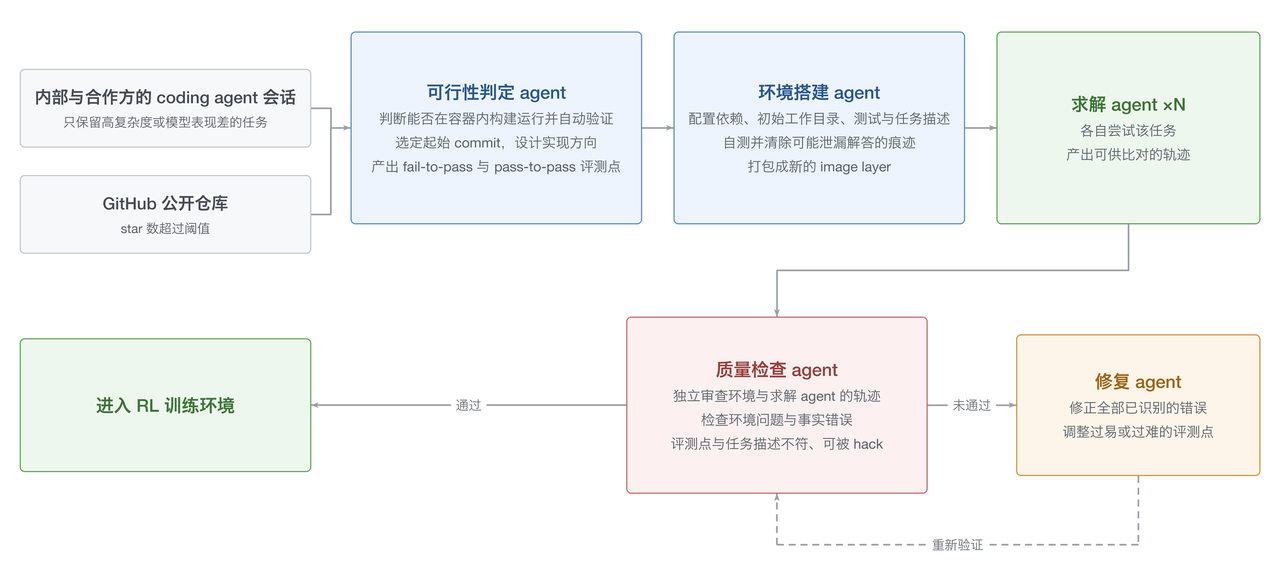
\includegraphics[width=0.98\linewidth,height=0.82\textheight,keepaspectratio]{images/DeepSeek-V4.1-Flash训练/doxcnie6JAV9yxPBFsV6nWKF1gc.png}\end{center}
\begin{enumerate}
\item 
% source-block: 109 doxcnepsGeVcHyKH6WCmHyhm3fb ordered
\textbf{可行性判定 agent：}判断项目能否在容器内完整构建运行、能否自动验证。通过之后选定起始轮次或 commit，设计若干足够复杂的实现方向，产出 \incode{fail-to-pass}与 \incode{pass-to-pass}，必要时联网获取外部资源。\par
\item 
% source-block: 110 doxcnoPFfCjsVKugaeb7bYjKAPc ordered
\textbf{环境搭建 agent：}在隔离容器内配置依赖、初始工作目录、测试代码与任务描述，先行自测，清除一切可能泄漏解答的痕迹，再打包成新的 image layer。\par
\item 
% source-block: 111 doxcni5TXLlB5A8YXkzSNEXeV0f ordered
\textbf{N 个求解 agent：}各自尝试该任务，为质量检查提供可供比对的轨迹。\par
\item 
% source-block: 112 doxcnUd9RopT31iXsN7i1L9iXUg ordered
\textbf{质量检查 agent（quality-inspection agent）} ：独立审查环境本身与求解 agent 的 trajectory，检查环境问题、事实错误、评测点与任务描述不符，以及 hackability 风险。\par
\item 
% source-block: 113 doxcnU3GtwVuaEsPkDtW9EeB2Ch ordered
\textbf{修复 Agent：}不通过则交给修复 agent，修正全部已识别的错误、调整过易或过难的评测点，重新进入验证。\par
\end{enumerate}

% source-block: 114 doxcnDyZ5pEV4L5sTqTpNIHYyTg heading3
\par\Needspace{8\baselineskip}\vspace{0.8em}\noindent \begin{tcolorbox}[boxrule=0pt,arc=3pt,colback=callOrange,left=3pt,right=3pt,top=2pt,bottom=2pt,before skip=0pt,after skip=0pt]{\zihao{3}\bfseries \textcolor{feishuBlue}{2.2}\ 合成任务上的 RL}\end{tcolorbox}\par\vspace{0.28em}

% source-block: 115 doxcngNLOOvUUpMfTAJDl7jRsSg heading4
\par\Needspace{8\baselineskip}\vspace{0.8em}\noindent \begin{tcolorbox}[boxrule=0pt,arc=3pt,colback=callGreen,left=3pt,right=3pt,top=2pt,bottom=2pt,before skip=0pt,after skip=0pt]{\zihao{4}\bfseries \textcolor{feishuBlue}{2.2.1}\ RL Scaling：训练算力 / scaffold 数量}\end{tcolorbox}\par\vspace{0.28em}

% source-block: 116 doxcn3sJx7U4DbS6XlihZ2W9gHc text
大规模异步 RL 在两个维度上扩展，training compute 和 scaffold（即外层 agent 框架，如 Claude Code、Codex）的数量。\par
\begin{itemize}
\item 
% source-block: 117 doxcnSk4bQrNr0TtvqW7v8m04yf bullet
单个 scaffold 内（DeepSeek Harness 的 Minimal 模式），四个 code benchmark 随 RL steps 的变化：\par
\end{itemize}

% source-block: 118 doxcnU8AQtDdCA7IGXGRyMJ759f image
\begin{center}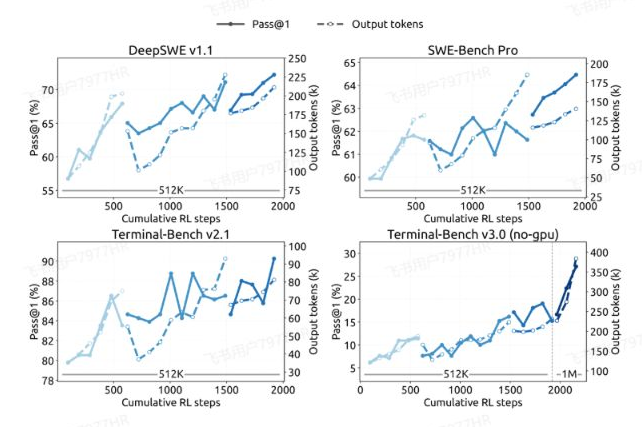
\includegraphics[width=0.98\linewidth,height=0.82\textheight,keepaspectratio]{images/DeepSeek-V4.1-Flash训练/doxcnU8AQtDdCA7IGXGRyMJ759f.png}\par 横轴下方标着上下文预算，前三段 run 的最大上下文都是 512K，Terminal-Bench v3.0 在最后一段扩到 1M 之后继续上升。\end{center}
\begin{itemize}
\item 
% source-block: 119 doxcnHN5TZbwECEEFnvVGhhKSbh bullet
跨版本与跨 scaffold 的联合训练，左边是多个 Claude Code 版本，右边是 OpenCode、Pi 与 DeepSeek Harness 的 Standard、PTC 模式：\par
\end{itemize}

% source-block: 120 doxcnq7t2JnGMTEGyCUeTOsXckg image
\begin{center}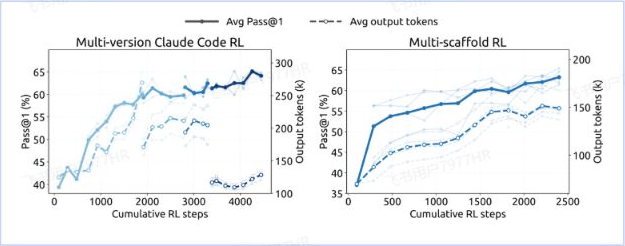
\includegraphics[width=0.98\linewidth,height=0.82\textheight,keepaspectratio]{images/DeepSeek-V4.1-Flash训练/doxcnq7t2JnGMTEGyCUeTOsXckg.png}\end{center}

% source-block: 121 doxcnchMxi08LFUji5nTX9qqELd heading4
\par\Needspace{8\baselineskip}\vspace{0.8em}\noindent \begin{tcolorbox}[boxrule=0pt,arc=3pt,colback=callGreen,left=3pt,right=3pt,top=2pt,bottom=2pt,before skip=0pt,after skip=0pt]{\zihao{4}\bfseries \textcolor{feishuBlue}{2.2.2}\ Model Merging}\end{tcolorbox}\par\vspace{0.28em}

% source-block: 122 doxcn13sJUoeOp1KF6ojl2dd4Wf text
\textbf{动机：单次 RL run 能利用的有效算力有限，}单个 run 训练到一定 step 之后继续加算力，收益递减。\par

% source-block: 123 doxcnvSD96c4Q1N0aRyIStxn27f text
\textbf{实现：用 model merging 初始化下一轮 RL，}把不同 scaffold 或不同配置的 run 的 checkpoint 合并，汇总沿不同优化路径得到的改进。上面两张图里断开的曲线段，就是 reinitialization 之后的后续 run，合并在 task performance 与 token efficiency 两侧都有进一步提升。\par

% source-block: 124 doxcnLU80kE2fiTUzQaw3GYtZcb heading3
\par\Needspace{8\baselineskip}\vspace{0.8em}\noindent \begin{tcolorbox}[boxrule=0pt,arc=3pt,colback=callOrange,left=3pt,right=3pt,top=2pt,bottom=2pt,before skip=0pt,after skip=0pt]{\zihao{3}\bfseries \textcolor{feishuBlue}{2.3}\ DSec（DeepSeek Elastic Compute）}\end{tcolorbox}\par\vspace{0.28em}

% source-block: 125 doxcnszeoU28z3g8Xy8agyku32f quote_container
\begin{feishuquote}

% source-block: 231 doxcn9ym2ierTzlgcT28gPKTeRd text
推荐前置阅读：\href{https://my.feishu.cn/wiki/RpoiwfvkCiR4dakQaP2cXAGWnMh?from=space_search}{执行与沙箱（Execution） }\par
\end{feishuquote}

% source-block: 126 doxcn1SCs42saqphiMC3AHQoGZf text
DSec（DeepSeek Elastic Compute）是 V3 到 V4 期间建设的 Agentic 训练与评测 sandbox 平台，V4.1 的 Agentic RL 训练需求达到数百万并发实例，瓶颈随之转移到 datacenter scalability、workload isolation、per-node density，以及 Agent 越界行为的遏制（containment of misbehavior）。\par

% source-block: 127 doxcnK5zpB9CBAajHNxp2hF9hhN heading3
\par\Needspace{8\baselineskip}\vspace{0.8em}\noindent \begin{tcolorbox}[boxrule=0pt,arc=3pt,colback=callOrange,left=3pt,right=3pt,top=2pt,bottom=2pt,before skip=0pt,after skip=0pt]{\zihao{3}\bfseries \textcolor{feishuBlue}{2.4}\ Controllable Reasoning Effort}\end{tcolorbox}\par\vspace{0.28em}

% source-block: 128 doxcnFhnX07HislKqpjMh8S2fHf text
\textbf{动机：}大模型存在 cost–quality trade-off，DeepSeek V4 的做法是训练并保存三个不同 RL 配置的 checkpoint 来提供 Non-think / Think High / Think Max 三档思考预算，档位离散保存权重。\par

% source-block: 129 doxcnGFsv1RB1GbGJFlsGIIYkxh text
\textbf{实现：}V4.1 在 RL 里引入标量 effort level $b\in\{1,\ldots,100\}$ 作为显式的 conditioning signal。以一行指令写在 system prompt 开头，single-turn reasoning 与 multi-turn agentic 任务都使用：\par

% source-block: 130 doxcn673uRvEhDrVG8q9xj2l3Pe code
% Code block omitted at user request.

% source-block: 131 doxcnyhjecU05iWLpbqugkeer1X text
因此单 checkpoint 由此可以沿学到的 cost–quality frontier 移动，训练只用有限个档位。\par

% source-block: 132 doxcnf3caD5bJhbcJevy2kxzTQd heading4
\par\Needspace{8\baselineskip}\vspace{0.8em}\noindent \begin{tcolorbox}[boxrule=0pt,arc=3pt,colback=callGreen,left=3pt,right=3pt,top=2pt,bottom=2pt,before skip=0pt,after skip=0pt]{\zihao{4}\bfseries \textcolor{feishuBlue}{2.4.1}\ 分组采样与长度惩罚}\end{tcolorbox}\par\vspace{0.28em}

% source-block: 133 doxcnwiKagF2sI89lDde1Olesod quote_container
\begin{feishuquote}

% source-block: 232 doxcnripdGrH8O9jLe7lZksMXEd text
\textbf{这里要解决的问题：}如何让同一个模型学会区分档位，同时又不让不同档位的回答互相比较（GRPO 的组相对优势不能混入 effort，否则优势计算会失去意义）。\par
\end{feishuquote}

% source-block: 134 doxcn75PYKn4sPM4KQ3Mp8bYPyg text
每个训练 prompt 在每个 effort 档位上各采样 $M_b$ 条回答：\par

% source-block: 135 doxcnT2JqL3pZJAASBJZDlJmAfg text
\bigmath{z_{b,j}\sim\pi_\theta(\cdot\mid x,b),\quad b\in\mathcal{B},\quad j=1,\ldots,M_b}
\begin{itemize}
\item 
% source-block: 136 doxcnjhWOLjFb3XO9wb9tk0qGaf bullet
$x$ 是训练 prompt，$\mathcal{B}$ 是训练使用的有限档位集合，$j$ 索引同一档位下的回答。\par
\item 
% source-block: 137 doxcnebWopRoGRiduHsk1t5Zlbb bullet
相同 $(x,b)$ 的回答构成一个 subgroup，reward 在 subgroup 内部 mean-centered 得到 group-relative advantage，不同档位的回答不直接比较。档位之间的行为差异不靠跨档位比较产生，而靠 reward 里的 length penalty 项随 $b$ 变化来诱导：\par
\end{itemize}

% source-block: 138 doxcnj5e8Ebi2zmGTov8MJ1w2Jf text
\bigmath{\begin{aligned}r_{b,j}^{\mathrm{len}}&=-\min\left\{C_{\max},\;k(b)\frac{\ell_{b,j}}{L_{\mathrm{norm}}}\right\},\\ k(b)&=k_0\exp\left(-\frac{b-b_{\min}}{\tau}\right),\qquad\tau=\lambda\overline{\Delta b}\end{aligned}}
\begin{itemize}
\item 
% source-block: 139 doxcnMCmL4Y7UopRDiPynS0qjFe bullet
$\ell_{b,j}$ 是 reasoning token 数量，$L_{\mathrm{norm}}$ 是参考长度，$C_{\max}$ 是单条 trajectory 扣分的上限。\par
\item 
% source-block: 140 doxcnLlnFZYnWJCSBDbeSmbqqgf bullet
$k_0$ 是最低档 $b_{\min}$ 处的 basic penalty coefficient，$\overline{\Delta b}$ 是训练档位的平均间距，$\lambda$ 控制衰减速率。\par
\item 
% source-block: 141 doxcnhvKO9alY9NG2SNEMuqYMUe bullet
$b$ 每增加 $\tau$，$k(b)$ 就乘以 $e^{-1}$。$k_0$ 决定整体压短推理的力度，$\tau$ 越小惩罚衰减越快。\par
\end{itemize}

% source-block: 142 doxcnQPqu0iePzfWbE3jGZZag0d heading3
\par\Needspace{8\baselineskip}\vspace{0.8em}\noindent \begin{tcolorbox}[boxrule=0pt,arc=3pt,colback=callOrange,left=3pt,right=3pt,top=2pt,bottom=2pt,before skip=0pt,after skip=0pt]{\zihao{3}\bfseries \textcolor{feishuBlue}{2.5}\ 异步后训练 Infra（Asynchronous Post-training Infrastructure）}\end{tcolorbox}\par\vspace{0.28em}

% source-block: 143 doxcnOeTXJFVAHQQE5ugSATp0Jh text
\textbf{动机：rollout 阶段的长尾是 RL 训练效率的主要瓶颈。}\par

% source-block: 144 doxcn8QuzOTR6QcLtjSRpiaaaId text
\textbf{实现：rollout 与 training 在同一批物理设备上 colocate 并分时执行。}每个任务只指定 in-flight 样本数上限，不需要手动在两个阶段之间分配资源。完整循环：\par

% source-block: 145 doxcnPWi3YSFM4A7OkSiCkOQgxc image
\begin{center}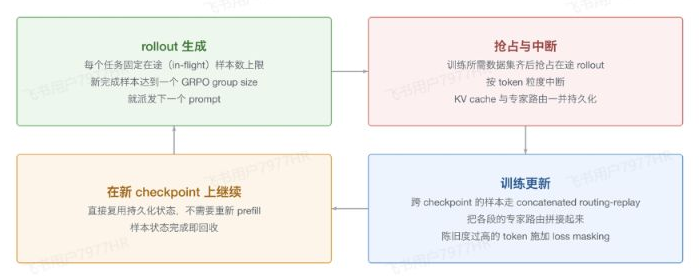
\includegraphics[width=0.98\linewidth,height=0.82\textheight,keepaspectratio]{images/DeepSeek-V4.1-Flash训练/doxcnPWi3YSFM4A7OkSiCkOQgxc.png}\end{center}

% source-block: 146 doxcnnuTYWalz0drAf6WG94g7Ve heading4
\par\Needspace{8\baselineskip}\vspace{0.8em}\noindent \begin{tcolorbox}[boxrule=0pt,arc=3pt,colback=callGreen,left=3pt,right=3pt,top=2pt,bottom=2pt,before skip=0pt,after skip=0pt]{\zihao{4}\bfseries \textcolor{feishuBlue}{2.5.1}\ dispatch 粒度}\end{tcolorbox}\par\vspace{0.28em}

% source-block: 147 doxcnmWmdUCKP20kI8FjqEq1Teb text
dispatch 粒度最终使用 sample-level，V4.1 消融测试过其他两种粒度：\par
\begin{itemize}
\item 
% source-block: 148 doxcne1Fa013wVQ2iBOYvyJZ6RU bullet
\textbf{Batch-level}：起始阶段多派发几个 batch，每轮训练之后补满一个 batch，结果训练指标剧烈震荡，说明这个粒度太粗。\par
\item 
% source-block: 149 doxcnFvoNGdzSUHIZrYw5n8RWHc bullet
\textbf{Prompt-level}：一个 GRPO 组完成之后派发一个新 prompt。结果是容易卡在组内的长尾样本上，难以平稳维持目标并发。\par
\item 
% source-block: 150 doxcnx8YsBUiLGfBNPmEhqS5AXM bullet
\textbf{Sample-level（最终方案）}：新完成的样本数一旦达到下一个 prompt 的 GRPO group size，就立刻派发该 prompt，无论这些样本来自哪些组，并发全程平稳。\par
\end{itemize}

% source-block: 151 doxcnHOkz8HTXMvVw6mBAcfAg9o heading4
\par\Needspace{8\baselineskip}\vspace{0.8em}\noindent \begin{tcolorbox}[boxrule=0pt,arc=3pt,colback=callGreen,left=3pt,right=3pt,top=2pt,bottom=2pt,before skip=0pt,after skip=0pt]{\zihao{4}\bfseries \textcolor{feishuBlue}{2.5.2}\ Length Bias 与 Off-Policy}\end{tcolorbox}\par\vspace{0.28em}

% source-block: 152 doxcnDyf9nGsJPeiCJ99zC55nU5 text
异步生成带来两个副作用分开处理：\par
\begin{itemize}
\item 
% source-block: 153 doxcnTWB9caTGNVUMi71UQSjmOd bullet
\textbf{Length bias（长度分布偏置）}：短序列先完成，会主导训练早期的 batch。dispatcher 按数据集限制 concurrency 调节稳态配比，再丢弃过早返回的短样本。\par
\item 
% source-block: 154 doxcnY30bESEApQnzUFSBMbm5gb bullet
\textbf{Off-policy}：部分或全部 token 由更早的 checkpoint 生成。调整 dispatch 逻辑与等待条件给最大 off-policy ratio 设上界，训练时再加 loss masking 剔除陈旧度过高的 token。\par
\end{itemize}

% source-block: 155 doxcnrwpSEBGJCAWTA1MpKPpyS4 text
需要 Infra 支持 token-level 中断，训练所需数据集齐之后在途样本立即停止。KV cache 与专家路由按 token 粒度持久化，换 checkpoint 后直接复用，省掉 re-prefill 开销。\par

% source-block: 156 doxcnHJtrlA9g3LtoPiM1lvhvjb heading3
\par\Needspace{8\baselineskip}\vspace{0.8em}\noindent \begin{tcolorbox}[boxrule=0pt,arc=3pt,colback=callOrange,left=3pt,right=3pt,top=2pt,bottom=2pt,before skip=0pt,after skip=0pt]{\zihao{3}\bfseries \textcolor{feishuBlue}{2.6}\ 大规模 OPD（Large-Scale On-Policy Distillation）}\end{tcolorbox}\par\vspace{0.28em}

% source-block: 157 doxcnqSH01Ql11KPFiDbkZHWtKg text
后训练的最后阶段是 full-vocabulary OPD，在全部 domain 的数据上训练，同样采用 asynchronous generation。方法脉络见 \href{https://my.feishu.cn/wiki/TaPYw0sGViHBFNkXdFIceLTWnEg}{\feiEmoji{📗}2026年基座模型中的 On-Policy Distillation 技术总结}。\par
\begin{itemize}
\item 
% source-block: 158 doxcnRiYCv5anMU4OKNjVFoOAle bullet
\textbf{40 个以上的 teacher}：各 domain 的训练过程不同，每个 domain 的最佳 teacher 可能来自模型的不同阶段。\par
\item 
% source-block: 159 doxcnuqpjed7aP348HUElwcxrSh bullet
\textbf{架构可异构}：teacher 之间、teacher 与 student 之间的架构允许不同。post-training infra 支持 teacher 数量不设上限，并以可忽略的代价在它们之间切换。\par
\item 
% source-block: 160 doxcnAE5nWFWxBYw3W53UXJkRhd bullet
\textbf{训练中动态重配（dynamic reconfiguration）}：持续跟踪模型能力并相应调整配方，包括 dataset mixture、各数据集的 concurrency limit、以及当前 active 的 teacher。\par
\end{itemize}

% source-block: 161 doxcnhy48ZBkjLWX5UPBl1mLsCd text

% source-block: 162 doxcnCqvIFbiU0L10PBlW5cCu5t heading2
\par\Needspace{8\baselineskip}\vspace{0.8em}\noindent \begin{tcolorbox}[boxrule=0pt,arc=3pt,colback=callRed,left=3pt,right=3pt,top=2pt,bottom=2pt,before skip=0pt,after skip=0pt]{\zihao{-2}\bfseries \textcolor{feishuBlue}{3.}\ 实验}\end{tcolorbox}\par\vspace{0.28em}

% source-block: 163 doxcnKXHBG3e88sPaA4bf2sR7vb heading3
\par\Needspace{8\baselineskip}\vspace{0.8em}\noindent \begin{tcolorbox}[boxrule=0pt,arc=3pt,colback=callOrange,left=3pt,right=3pt,top=2pt,bottom=2pt,before skip=0pt,after skip=0pt]{\zihao{3}\bfseries \textcolor{feishuBlue}{3.1}\ Post-Training 模型主实验}\end{tcolorbox}\par\vspace{0.28em}

% source-block: 164 doxcnXxGyGkCckrux3ZvCAsHGPe image
\begin{center}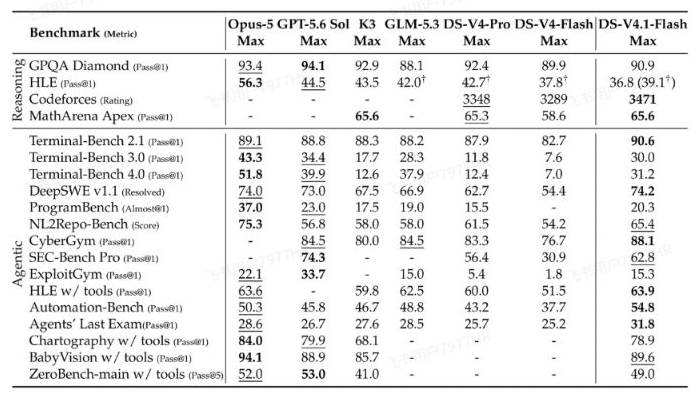
\includegraphics[width=0.98\linewidth,height=0.82\textheight,keepaspectratio]{images/DeepSeek-V4.1-Flash训练/doxcnXxGyGkCckrux3ZvCAsHGPe.png}\end{center}
\begin{itemize}
\item 
% source-block: 165 doxcnxVuZRufeGR5OWHIRw7vHcc bullet
\textbf{Coding Agent 是增量最大}：在 DeepSWE v1.1 是 74.2，Terminal-Bench 2.1 是 90.6。\par
\item 
% source-block: 166 doxcn384Ko7fS3lpBeICi4wldsf bullet
\textbf{Terminal-Bench 3.0 / 4.0 仍然落后}：在新 agentic benchmark 仍然落后闭源模型。\par
\item 
% source-block: 167 doxcnQaXBKDSHxB5ypd4qT9bp0c bullet
\textbf{网络安全能力}：CyberGym 88.1，SEC-Bench Pro 62.8 仍低于 GPT-5.6 Sol 的 74.3。\par
\end{itemize}

% source-block: 168 doxcn5Z2Tx0t0c0Z8bwG891DtNg heading3
\par\Needspace{8\baselineskip}\vspace{0.8em}\noindent \begin{tcolorbox}[boxrule=0pt,arc=3pt,colback=callOrange,left=3pt,right=3pt,top=2pt,bottom=2pt,before skip=0pt,after skip=0pt]{\zihao{3}\bfseries \textcolor{feishuBlue}{3.2}\ Reasoning Effort 的边际收益}\end{tcolorbox}\par\vspace{0.28em}

% source-block: 169 doxcnfhuFRr9AOKqjtcekbAp8ye text
Reasoning Effort 从 25 提升到 100，Pass@1 与 output length 同步上升：\par

% source-block: 170 doxcn0UQ2wnqKqcgZEZjDapCJVf image
\begin{center}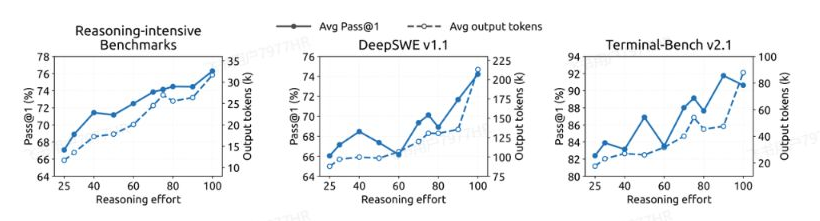
\includegraphics[width=0.98\linewidth,height=0.82\textheight,keepaspectratio]{images/DeepSeek-V4.1-Flash训练/doxcn0UQ2wnqKqcgZEZjDapCJVf.png}\end{center}

% source-block: 171 doxcnHQE1KmFkVdeRkrQwwv9xIb text
\textbf{收益前置（front-loaded）}：Reasoning Effort 从 60 提升到 80 这一段已经恢复到最高档大部分的 accuracy，继续提升到 100 会让 agent trajectory 长出 1.6～1.8 倍，只换来边际提升。这意味着日常 Agentic 使用取中等档位更划算，最高档留给最难的任务。\par

% source-block: 172 doxcnXv2uFjEi1aMgqbMAwLrIPg text
在 single-response reasoning 上学到的 effort 控制同样迁移到了 long-horizon agentic trajectory，八个推理 benchmark 的逐项曲线：\par

% source-block: 173 doxcnvT9wMYqe4uE2LLgOx9sNqf image
\begin{center}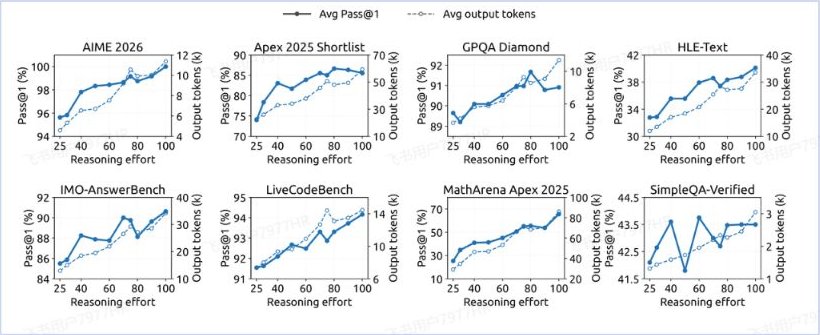
\includegraphics[width=0.98\linewidth,height=0.82\textheight,keepaspectratio]{images/DeepSeek-V4.1-Flash训练/doxcnvT9wMYqe4uE2LLgOx9sNqf.png}\end{center}

% source-block: 174 doxcnDwrQoqSALFklR7DuFRJA8b heading3
\par\Needspace{8\baselineskip}\vspace{0.8em}\noindent \begin{tcolorbox}[boxrule=0pt,arc=3pt,colback=callOrange,left=3pt,right=3pt,top=2pt,bottom=2pt,before skip=0pt,after skip=0pt]{\zihao{3}\bfseries \textcolor{feishuBlue}{3.3}\ Scaffold 适配鲁棒性}\end{tcolorbox}\par\vspace{0.28em}

% source-block: 175 doxcnANIvHUCwp9csSlvyIrboDf text
模型接入到 agent 框架里，不同的 system prompt、tool definition、context management、interaction protocol 可能造成模型能力可能大幅退化。这组实验保持模型 checkpoint、decoding 配置、任务集完全一致，只换外层 harness，覆盖六个 scaffold 家族的八个配置：\par

% source-block: 176 doxcnKw3pfRgEmuWvNIhgEOh0Bb image
\begin{center}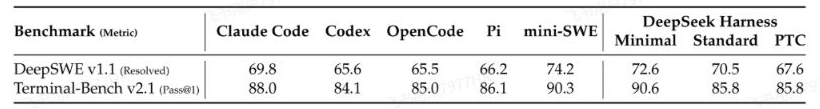
\includegraphics[width=0.98\linewidth,height=0.82\textheight,keepaspectratio]{images/DeepSeek-V4.1-Flash训练/doxcnKw3pfRgEmuWvNIhgEOh0Bb.png}\end{center}
\begin{itemize}
\item 
% source-block: 177 doxcn1duURgo8lzbMLdlK30W5Se bullet
DeepSWE v1.1 落在 65.5 到 74.2 之间，八个配置全部使用 Max effort（100）。\par
\item 
% source-block: 178 doxcnuI6CtNNEoovDxAjuQSJm0e bullet
两项的最高分并不在同一个 scaffold 上：DeepSWE 最高是 mini-SWE 的 74.2，Terminal-Bench 最高是 DeepSeek Harness 的 90.6。\par
\item 
% source-block: 179 doxcnE84y0fVY6TNzoj2P01JbEe bullet
effort 在不同 scaffold 上的表现：\par
\end{itemize}

% source-block: 180 doxcnSaOYnySZWOvJZaFUdzYA7b image
\begin{center}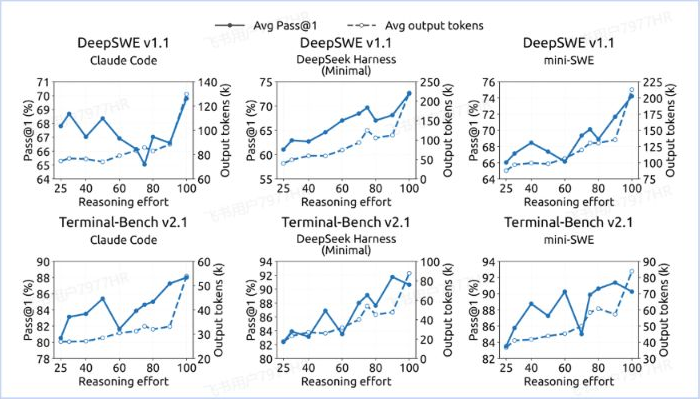
\includegraphics[width=0.98\linewidth,height=0.82\textheight,keepaspectratio]{images/DeepSeek-V4.1-Flash训练/doxcnSaOYnySZWOvJZaFUdzYA7b.png}\end{center}

% source-block: 181 doxcnQTZVJWgGr7u9EFiOkLvZPd text

% source-block: 182 doxcnFRf8XtXyMkpSiFqW4FRtuf heading3
\par\Needspace{8\baselineskip}\vspace{0.8em}\noindent \begin{tcolorbox}[boxrule=0pt,arc=3pt,colback=callOrange,left=3pt,right=3pt,top=2pt,bottom=2pt,before skip=0pt,after skip=0pt]{\zihao{3}\bfseries \textcolor{feishuBlue}{3.4}\ Multi-Agent：Agent Team 实验}\end{tcolorbox}\par\vspace{0.28em}
\begin{itemize}
\item 
% source-block: 183 doxcnblKQyij99QqoIQ2PsMdkWK bullet
\textbf{组织方式}：lead agent 通过 \incode{spawn\_teammate} 异步创建具名的持久 teammate，全部 agent 共享一份 repository checkout，改动彼此立即可见。\par
\item 
% source-block: 184 doxcnmm8bW7j2Ew5NjvG2m1rCve bullet
\textbf{奖励构成}：task performance，加上鼓励 delegation 与 inter-agent communication 的 collaboration bonus，再减去 derived-latency penalty。\par
\item 
% source-block: 185 doxcnCj4SRbPumXKfLxcAuLVZYg bullet
\textbf{Derived latency}：把执行事件与协作依赖表示成有向无环图（DAG），按固定 prefill、decode 速率从 token 数折算成本，加上实测的 tool execution time，取 critical path 长度。鼓励有效并行、惩罚无谓的串行与同步，同时对服务端的 batching 与排队延迟不敏感。\par
\end{itemize}

% source-block: 186 doxcnJypV1UxZN0CFuJIGrXrzsh image
\begin{center}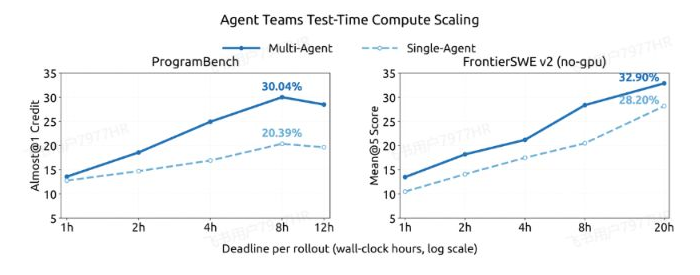
\includegraphics[width=0.98\linewidth,height=0.82\textheight,keepaspectratio]{images/DeepSeek-V4.1-Flash训练/doxcnJypV1UxZN0CFuJIGrXrzsh.png}\end{center}
\begin{itemize}
\item 
% source-block: 187 doxcnIq2udhIgtD3llUc1oRIjzg bullet
ProgramBench 的高置信子集（参考解在隐藏测试集上通过率不低于 95\% 的 172 道题），multi-agent 的 Almost@1（得分不低于 0.95 的 rollout 占比）从 1 小时的 13.59\% 升到 8 小时的峰值 30.04\%，single-agent 同期是 12.79\% 到 20.39\%。\par
\item 
% source-block: 188 doxcntz6iDYmL2vELVT0u2zTwnb bullet
FrontierSWE v2 的 no-GPU 子集（不需要 GPU 的那部分任务）上，multi-agent 的 Mean@5 从 1 小时的 13.50\% 升到 20 小时的 32.90\%，single-agent 是 10.50\% 到 28.20\%。\par
\end{itemize}

% source-block: 189 doxcnEQW24XINlaWkBCUFzSTDcg text
两个 benchmark 上 multi-agent 在每一个 deadline 上都优于 single-agent。\par

\end{document}
